\newpage % Rozdziały zaczynamy od nowej strony.
\section{Wyniki pracy}
Niniejszy rozdział prezentuje główne wyniki uzyskane w trakcie badania i zawiera w sobie podsumowanie przeprowadzonych eksperymentów. Omówione zostaną w nim wszystkie uzyskane rezultaty, które pozwalają na ocenę czy sztuczne sieci neuronowe mogą być stosowane z powodzeniem w obszarze regulacji. Na początku zaprezentowany zostanie sposób generacji danych, poczynione założenia i sposób działania regulacji opartej o sieć neuronową. Kolejno wybrana zostanie optymalna liczba neuronów warstwy ukrytej pozwalająca na minimalizację funkcji celu z zachowaniem ogólności rozwiązania. W kolejnej części zbadany zostanie wpływ zastosowania redukcji sieci na osiągane przez nią rezultaty. Po wybraniu optymalnej struktury i pełnym wytrenowaniu sieci zbadamy jak poradzi sobie z regulacją obiektów, które nie znalazły odzwierciedlenia w przykładach uczących. Pod koniec rozdziału sformułowane zostaną ogólne wnioski i uwagi płynące z całości eksperymentów, które znajdą również swoje odzwierciedlenie w późniejszym podsumowaniu pracy.

\subsection{Generacja danych}
Niezbędnym krokiem przed przystąpieniem do trenowania sieci neuronowej jest generacja danych, na podstawie których sieć następnie zostanie nauczona. Celem pracy jest zweryfikowanie zdolności adaptacji sieci do działania jako regulator DMC. Kierując się tym założeniem oczywistym wydaje się wygenerowanie danych uczących na podstawie symulacji przeprowadzonych z wykorzystaniem rzeczywistego regulatora DMC. Praca ma jedynie charakter porównawczy, a więc za najogólniejszy przykład regulacji możemy wybrać dostosowanie wyjścia obiektu regulacji do jednokrotnego skoku wartości zadanej. Jako obiekt regulacji wybrany został w tej części układ opisany we wcześniejszej części pracy, który identyfikujemy poprzez następujące parametry: \( T_1=5, \, T_2=2, \, K=1, \, T_d=0 \). Wybór dokonany został w sposób arbitralny, gdyż przeprowadzenie eksperymentów z wykorzystaniem dowolnego innego układu pozwala osiągnąć zbliżone rezultaty i wyciągnąć analogiczne wnioski.
\par Na tym etapie należy podjąć decyzję odnośnie wartości na podstawie, których sieć neuronowa dokonywać będzie regulacji. Kierując się analogią do klasycznych metod za dobrą praktykę wybrano sterowanie na podstawie wartości uchybu regulacji oraz aktualnej wartości zadanej. W trakcie przeprowadzanych eksperymentów długość symulacji wynosi 40 okresów jako okres, po którym układ regulowany za pomocą regulatora DMC osiąga pełną stabilność. Na tej podstawie do sterowania za pomocą sieci wybrane zostało 30 wartości uchyby regulacji oraz aktualna wartość zadana. Wyjściem sieci jest oczywiście pojedynczy sygnał sterujący co stanowi pewną modyfikację względem algorytmu DMC gdzie, w każdej iteracji wyznaczana jest zmiana sterowania. Opisana modyfikacja stanowi jedynie szczegół implementacyjny, który nie wpływa na wyniki osiągane przez sieć.
\par Jak zostało już opisane w części teoretycznej dane uczące i weryfikujące generowane są w sposób niezależny na podstawie oddzielnych przebiegów regulacji. Dzięki takiej strategi mamy pewność, że sieć zostanie przetestowana pod kątem ogólnej aproksymacji algorytmu OBD, a nie jedynie wybranych przebiegów regulacji. Kolejno przeprowadzone zostały eksperymenty polegające na wyznaczeniu przebiegu regulacji predykcyjnej dla jednostkowych skoków wartości zadanej z zakresu od 1 do 10 z krokiem co 0,1. Przebiegi regulacji podzielone zostały na dane uczące i weryfikujące w stosunku 75\% - 25\% . Po próbkowaniu dla każdej iteracji zbiór uczący ostatecznie składa się z 3015 przykładów, natomiast weryfikujący z 1035.
\par Ostatnim krokiem przed przystąpieniem do procedury uczenia sieci neuronowej było wymagane przeskalowanie zbioru danych. Jak już zostało wskazane z uwagi na sigmoidalną funkcję aktywacji koniecznym było napisanie modułu transformującego  zarówno dane wejściowe jak i wyjściowe sieci do zakresu \( (-1,1) \). Warto zauważyć, że skalowanie wartości wejściowych i wyjściowych przebiega niezależnie oraz moduł skalujący umożliwia odwrotne skalowanie wyjścia sieci, które następnie wykorzystywane jest w trakcie regulacji. Stanowi to istotne ograniczenie w działaniu sieci, a mianowicie sieć jest w stanie regulować tylko układy dla których pożądane wartości sterowania zawierają się w zakresie reprezentowanym przez dane wykorzystane do nauki sieci.  

\subsection{Wybór struktury sieci}
Pierwszym krokiem prowadzącym do wyselekcjonowania optymalnej architektury sieci jest wybór jej struktury. Liczba neuronów w warstwie wejściowej i wyjściowej ściśle zależy do charakterystyki problemu, a więc wygenerowanych uprzednio danych. Szczególną uwagę należy poświęcić za to prawidłowemu doborowi liczby neuronów w warstwie ukrytej. W tym celu przeprowadzono eksperyment pokazujący wartość kwadratowej funkcji kosztu w zależności od liczby neuronów w warstwie ukrytej. Przetestowano wartości z zakresu od 5 do 200 neuronów, a wyniki symulacji zaprezentowane zostały na Rysunku 5.1. 
\par Na tym etapie trenowania sieci neuronowej głównym celem jest minimalizacja funkcji kosztu na danych uczących z uwagi na  stosowany w kolejnym kroku algorytm OBD. W ramach zaprezentowania pełniejszego obrazu na Rysunku 5.2. przedstawiona została analogiczna symulacja z wykorzystaniem danych weryfikujących (testowych). Widzimy, że wyniki obu eksperymentów są ze sobą niezwykle spójne. Obserwacja ta potwierdza intuicję, gdyż zarówno zbiór danych uczących jak i weryfikujących wygenerowany został na podstawie analogicznych symulacji, w czasie których modyfikowana była jedynie wartość zadana. 

\begin{figure}[!h]
  \label{fig:Koszt-liczba-neuronow-treningowe}
  \centering 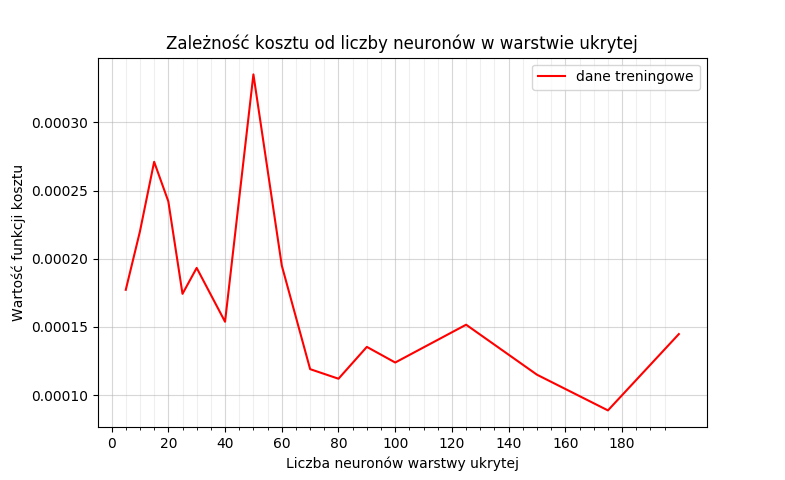
\includegraphics[width=0.7\linewidth]{cost_neuron_number_train.png}
  \caption{Zależność kosztu od liczby neuronów w warstwie ukrytej - dane treningowe}
\end{figure}

\begin{figure}[!h]
  \label{fig:Koszt-liczba-neuronow-testowe}
  \centering 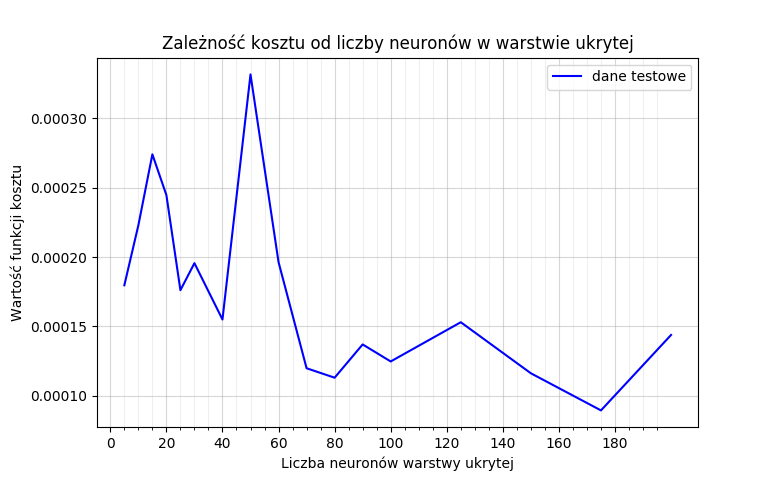
\includegraphics[width=0.7\linewidth]{cost_neuron_number_test.png}
  \caption{Zależność kosztu od liczby neuronów w warstwie ukrytej - dane testowe}
\end{figure}

\par Analiza wykresów dostarcza kilku istotnych obserwacji. Pierwszą z nich jest to, że nawet niezwykle prosta struktura jaką jest sieć neuronowa o jedynie 5 neuronach w warstwie ukrytej jest w stanie zadowalająco dobrze nauczyć się postawionego przed nią zadania regulacji. Warto jednak zwrócić uwagę, że sieci o małej liczbie neuronów wykazują się wysoką niestabilnością przez co rezultaty przez nie osiągane mogą różnić się pomiędzy kolejnymi próbami. Po kilkukrotnym powtórzeniu eksperymentu zaobserwowano wyeliminowanie problemu dla sieci neuronowych z liczbą neuronów w warstwie ukrytych przekraczającą 100. Na tej podstawie do dalszych eksperymentów wybrana została sieć o 150 neuronach. 
\par Po wybraniu optymalnej struktury sieci należy zwrócić uwagę na zależność kosztu od liczby epok, przez które sieć jest trenowana. Pozwoli to na weryfikację wartości granicznej gradientu funkcji celu, która stanowi warunek wyjścia dla metody uczenia sieci. Początkowa kryterium wyjścia ustalone zostało na poziomie \( 10^{-5} \) co oznacza, że jeżeli gradient funkcji kosztu przez 3 kolejne iteracje jest mniejszy od zadanej wartości algorytm przerywa uczenie sieci. Eksperyment ten możemy przeprowadzić zdejmując wcześniejsze ograniczenie i sprawdzając jak zmienia się funkcja kosztu dla 300 iteracji algorytmu (epok). Wykres przedstawiający wspomnianą zależność zaprezentowany został na Rysunku 5.3 natomiast na Rysunku 5.4 przedstawione zostały te same dane ale z uciętymi 50 początkowymi wartościami w celu dokładniejszej prezentacji wyników czytelnikowi.
\par Należy zwrócić uwagę, że już po 40 epokach wyniki osiągane przez sieć można uznać za satysfakcjonujące, jednak w dalszym ciągu obserwujemy stosunkowo duże wahania wartości funkcji kosztu i nie osiągamy pełnej stabilności. Okresowe wahania ustają po około 150 iteracjach i po takiej liczbie epok możemy uznać, że redukcja funkcji kosztu jest nieznaczna. Dzięki wielokrotnemu  powtórzeniu eksperymentu oraz przetestowaniu różnych wartości kryterium wyjścia za zadowalająca wartość przyjęto \( 5*10^{-6} \), co stanowi redukcję wcześniej przyjętego poziomu o połowę.

\begin{figure}[!h]
  \label{fig:Koszt-liczba-epok}
  \centering 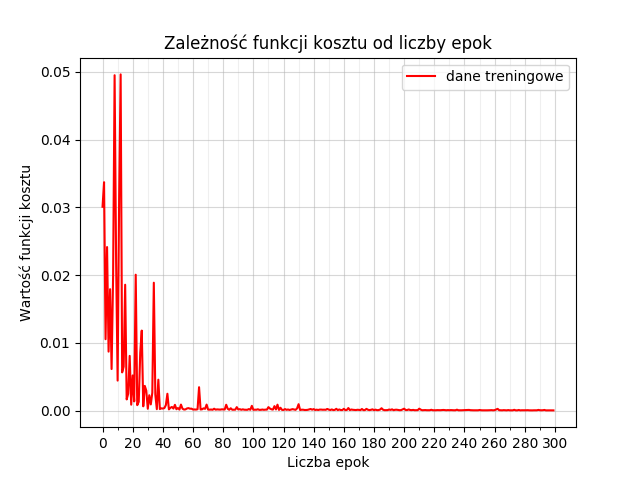
\includegraphics[width=0.7\linewidth]{cost_epoch_150.png}
  \caption{Zależność kosztu od liczby epok dla sieci z 150 neuronami}
\end{figure}

\begin{figure}[!h]
  \label{fig:Koszt-liczba-epok-zoom}
  \centering 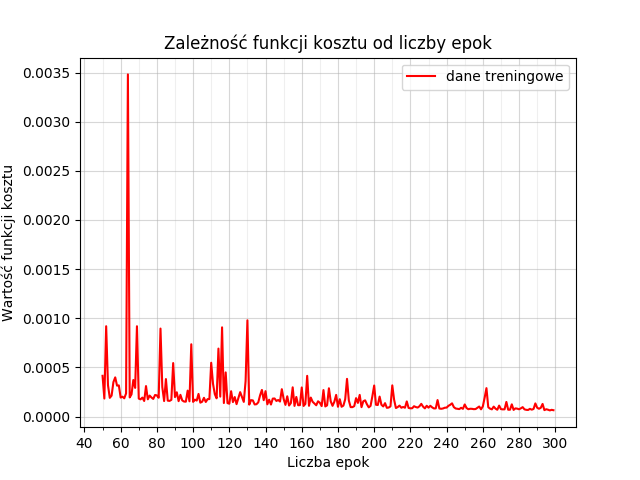
\includegraphics[width=0.7\linewidth]{cost_epoch_150_zoom.png}
  \caption{Zależność kosztu od liczby epok dla sieci z 150 neuronami (ucięte wartości początkowe)}
\end{figure}

\par Na tym etapie dokonano wstępnego porównania klasycznej metody DMC z regulatorem opartym o w pełni wytrenowaną sieć neuronową, jeszcze przed zastosowaniem algorytmu OBD. W tym celu przeprowadzono następujący eksperyment, sprawdzono zdolność dostosowania wyjścia obiektu do jednokrotnego skoku wartości zadanej. Za miarę jakości regulacji przyjęto powszechnie stosowany błąd średniokwadratowy \emph{(ang. mean squared error MSE)}. Sprawdzono zdolność dostosowania wyjścia obiektu do 5 różnych wartości zadanych: 2,5 ; 4 ; 5,21 ; 6,1 ; 7. Wartości dobrane zostały w taki sposób aby sprawdzić zachowanie regulatora na całym zakresie reprezentowanym przez dane uczące. Eksperyment został powtórzony 10-krotnie aby wyeliminować wpływ pewnej losowości, jaką charakteryzuje się proces uczenia sieci neuronowej. Uśrednione wartości błędu MSE dla każdej z wartości zadanej zaprezentowane zostały w tabeli 5.1.
\begin{table}[!h] \label{tab:tabela1} \centering
\caption{Porównanie MSE dla w pełni wytrenowanej sieci}
\begin{tabular} {| c | c | c |} \hline
    Wartość zadana & MSE sieć & MSE DMC \\ \hline\hline
    2,5 & 0,606 & 0,592 \\ \hline
    4 & 1,499 & 1,517 \\ \hline
    5,21 & 2,518 & 2,573 \\ \hline
    6,1 & 3,457 & 3,527 \\ \hline
    7 & 4,579 & 4,645 \\ \hline
    Średnia & 2,532 & 2,571 \\ \hline
    
\end{tabular}
\end{table}
Analizując przedstawioną tabele możemy stwierdzić, że sieć neuronowa poradziła sobie z zadaniem regulacji, które zostało przed nią postawione. Co więcej dla czterech z pięciu przypadków obserwujemy mniejszą wartość błędu MSE niż dla regulatora DMC. Przypadek dla którego klasyczny regulator poradził sobie nieznacznie lepiej dotyczył najmniejszej wartości zadanej co może świadczyć o tym, że w obrębie względnie małych zmian wartości zadanych regulacja oparta o sieć neuronową charakteryzuje się mniejszą precyzją. Warto również zwrócić uwagę na to, że dla wartości zadanej wynoszącej 5,21 sieć w pełni poradziła sobie z zadaniem regulacji przed nią postawionym. Jest to o tyle ważne, że dana wartość nie była reprezentowana w danych uczących co udowadnia, że sieć neuronowa nauczona została ogólnego zadania regulacji, a nie jedynie przebiegów dla pojedynczych wartości zadanych, które znalazły odzwierciedlenie w przykładach trenujących. 

\par Warto pokazać również przebieg jednej z przykładowych regulacji, na podstawie których wyznaczona została Tabela 5.1. Zaprezentowane zostaną przebiegi dla wartości zadanej 5,21 z przyczyn opisanych w poprzednim paragrafie. Na Rysunku 5.5 widzimy regulację z wykorzystaniem sieci neuronowej dla wybranej wartości zadanej, natomiast Rysunek 5.6 pokazuje referencyjny przebieg uzyskany z wykorzystaniem regulatora DMC. Dokonując porównania dwóch wykresów możemy stwierdzić, że przebiegi wyjścia obiektu dla dwóch różnych regulatorów są do siebie zbliżone. Warto zauważyć, że regulacja z wykorzystaniem sieci neuronowej charakteryzuje się mniejszą stabilnością sygnału sterującego. Z cała pewnością jest to istotne ograniczenie, które jednak może potwierdzać zauważoną zależność w trakcie przeglądu literatury, przykłady praktycznego zastosowania sieci neuronowej w regulacji dotyczą jedynie wysoce dynamicznych obiektów. Pełnej weryfikacji postawionej tezy będzie można jednak dokonać po przetestowaniu uproszczonej sieci neuronowej.

\begin{figure}[!h]
  \label{fig:sim-net-5}
  \centering 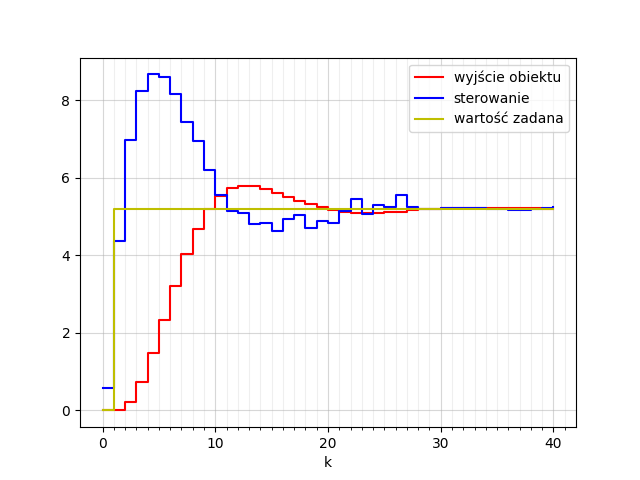
\includegraphics[width=0.7\linewidth]{regulation_net_5.png}
  \caption{Regulacja do wartości zadanej 5,21 - wytrenowana sieć neuronowa}

  \vspace*{\floatsep}% https://tex.stackexchange.com/q/26521/5764

  \label{fig:sim-dmc-5}
  \centering 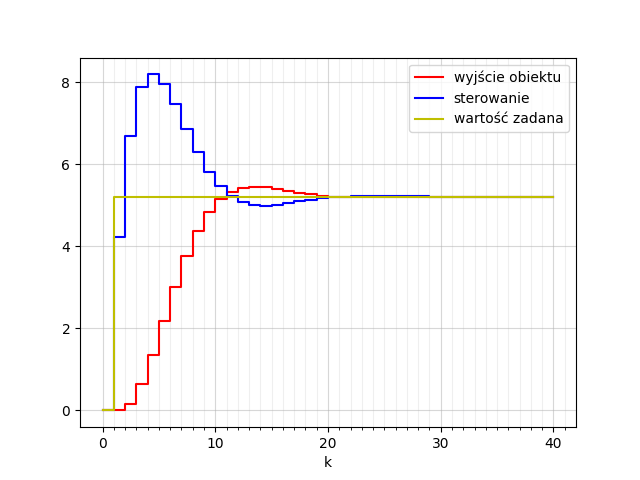
\includegraphics[width=0.7\linewidth]{regulation_DMC_5.png}
  \caption{Regulacja do wartości zadanej 5,21 - DMC}
\end{figure}

\par Przeprowadzony eksperyment wskazuje również na zasadność ustalenia kryterium wyjścia na wartość \( 5*10^{-6} \). W trakcie 10 powtórzeń uczenie sieci kończyło się w zakresie od 126 do 258 iteracji, po których uśredniony koszt wynosił 0,00012 z odchyleniem standardowym wynoszącym \( 2,9*10^{-5} \). Są to rezultaty, które możemy uznać za satysfakcjonujące przed przystąpieniem do procedury redukcji sieci.

\subsection{Zastosowanie algorytmu OBD}
Jak już zostało wskazane w rozdziale z opisem teoretycznym zastosowanie algorytmu OBD wymaga wcześniejszego osiągnięcia minimum funkcji kosztu na danych uczących. Z tego względu algorytm OBD może zostać zastosowany do sieci neuronowej stanowiącej wynik prac opisanych w poprzednim podrozdziale. Zgodnie z procedurą opisaną w sekcji 3.2.3 upraszczanie sieci neuronowej następuje w wersji iteracyjnej co oznacza, że w każdej kolejnej iteracji algorytmu redukowana będzie o jedna waga więcej. Jest to stosunkowo długa procedura gdyż wykorzystywana w pracy architektura składa się z 4800 połączeń między-neuronowych i jest to jednocześnie długość pętli algorytmu OBD. W każdym kroku należy również ponownie douczyć sieć aby spełniony był warunek o osiągnięciu minimum funkcji celu. Z tego względu czas obliczeniowy algorytmu wykonywanego na komputerze osobistym może wynieść nawet do kilku godzin, a wielokrotne powtarzanie procedury może okazać się niedogodne. Warto zauważyć również, że przycinanie stosowane jest dla wszystkich wag jednocześnie bez rozróżnienia na to pomiędzy, którymi warstwami sieci występują.
\par Kluczowym dla ostatecznej architektury jest prawidłowy wybór kryterium wyjścia z pętli algorytmu OBD. Istotnym jest wybór liczby upraszczanych wag, która pozwoli na zwiększenie zdolności generalizacji danego zadania. Jednocześnie należy pamiętać o tym, że redukcja zbyt dużej ilości połączeń może znacząco zaburzyć działanie sieci i drastycznie zwiększyć popełniany przez nią błąd. Optymalnym wyborem jest przeprowadzenie procedury OBD z wykorzystaniem danych uczących natomiast uzależnienie kryterium wyjścia od wartości funkcji kosztu dla danych weryfikujących. Zależy nam na minimalizacji wskazanego kosztu przy jednoczesnym zapewnieniu stabilnego działania sieci. Zdefiniowanie odpowiedniej miary a priori może okazać się niezwykle trudnym zadaniem dlatego pomocnym będzie eksperyment zastosowania procedury upraszczania sieci na całym dostępnym zakresie parametrów. W ten sposób  wyznaczymy zależność funkcji kosztu od liczby zredukowanych wag sieci neuronowej. Wyniki eksperymentu zaprezentowane zostały na rysunkach 5.7 oraz 5.8, które prezentują wykres funkcji kosztu dla kolejno danych testowych i treningowych. Na obu wykresach zakres prezentowanych wyników ograniczony został do 4700 początkowych pętli algorytmu, powyżej tej wartości następuje gwałtowny wzrost funkcji kosztu co przekłada się na wypłaszczenie pozostałej części przebiegu. W konsekwencji uniemożliwiłoby to prawidłową interpretację uzyskach rezultatów.

\begin{figure}[!h]
  \label{fig:Koszt-OBD-full-test}
  \centering 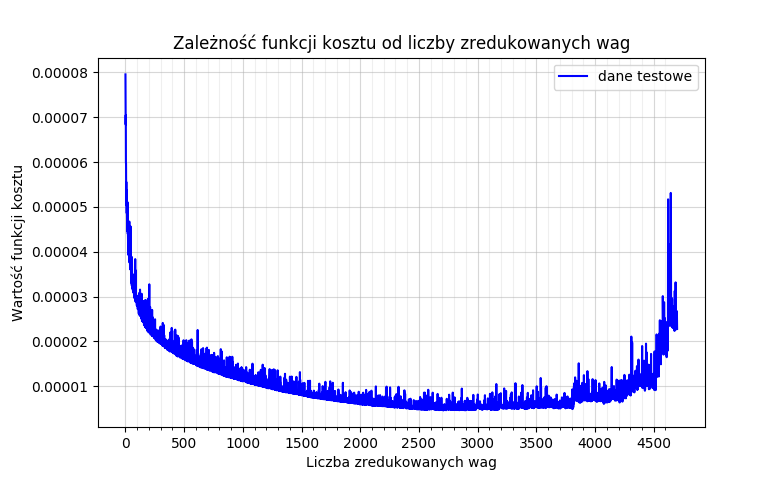
\includegraphics[width=0.7\linewidth]{cost_OBD_full_test.png}
  \caption{Zależność funkcji kosztu od liczby zredukowanych wag - dane testowe}

  \vspace*{\floatsep}% https://tex.stackexchange.com/q/26521/5764

 \label{fig:Koszt-OBD-full-train}
  \centering 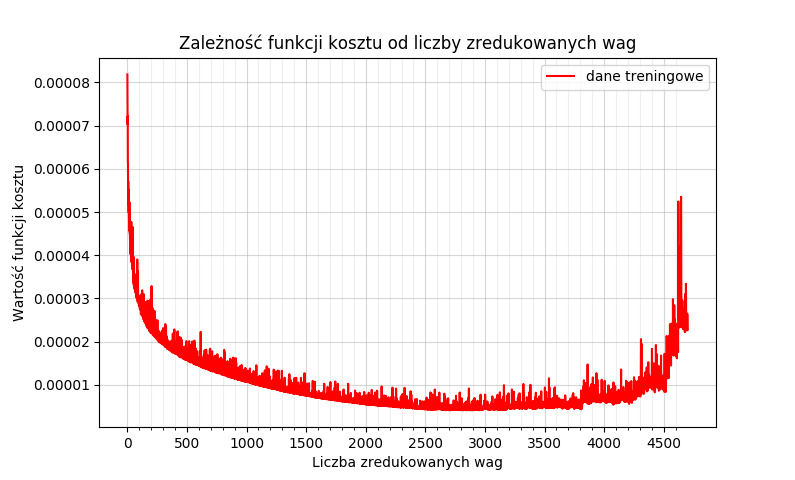
\includegraphics[width=0.7\linewidth]{cost_OBD_full_train.png}
  \caption{Zależność funkcji kosztu od liczby zredukowanych wag - dane treningowe}
\end{figure}

\par Główną uwagę należy zwrócić na wykres dla danych testowych gdyż to minimalizacja funkcji kosztu popełnianego na tym zestawie danych jest podstawowym zadaniem algorytmu OBD. Warto jednak zauważyć, że podobnie jak to miało miejsce w przypadku badania wpływu liczby neuronów warstwy ukrytej na funkcję kosztu, tak i tutaj przebiegi funkcji dla danych treningowych i testowych są praktycznie identyczne. Jest to jednak zależność, której należało się spodziewać na podstawie wcześniejszych obserwacji. Istotnym z punktu widzenia pracy jest fakt, że zastosowanie procedury przycinania sieci w istotny sposób wpływa na redukcję wartości kosztu. W przypadku naszego eksperymentu obserwowaliśmy prawie ośmiokrotny spadek analizowanej statystki. Wprawdzie możliwe było by osiągnięcie mniejszego bazowego kosztu dzięki wydłużeniu początkowej liczby epok, przez które trenowana była sieć jednak jak wykazaliśmy wcześniej nie można oczekiwać, aż tak znacznej redukcji jaką obserwujemy w trakcie procedury przycinania. Istotnym jest również fakt, że w czasie douczania sieci neuronowej po każdej kolejnej redukcji stosowane było takie samo kryterium wyjścia jak w początkowym etapie. W trakcie trwania całego eksperymentu liczba epok, po której dotrenowanie było zakańczane nie przekroczyła 50. Na tej podstawie należy stwierdzić, że algorytm OBD w istotny sposób przyczynia się do redukcji funkcji kosztu zarówno dla danych testowych jak i treningowych, a jego zastosowanie powinno przyczynić się do większej stabilności regulacji. 
\par Analizując Rysunki 5.7 oraz 5.8 należy stwierdzić, że pomimo osiągnięcia zadowalających rezultatów, na całym przebiegu funkcji występują zauważalne oscylacje pomiędzy kolejnymi iteracjami. Powoduje to, że zdefiniowanie kryterium wyjścia opartego na gradiencie funkcji staje się niestabilne i nie pozwala na osiągnięcie zadowalającej liczby zredukowanych wag. Z tego względu zastosowana została inna strategia. Na podstawie zaprezentowanych przebiegów widzimy, że funkcja kosztu maleje aż zredukowane zostanie około 2500 parametrów czyli nieco ponad połowa wag sieci. Dalsze upraszczanie prowadzi do utrzymania kosztu na prawie stałym poziomie aż przycięte zostanie zbyt dużo parametrów co w rezultacie uniemożliwia sieci generalizację problemu przed nią postawionego. Dla danych testowych minimum wynoszące \( 4,614*10^{-6} \) osiągnięte zostało po przycięciu 2708 wag. Kierując się powyższymi obserwacjami zasadnym jest ustalenie kryterium zakończenia procedury przycinania sieci na redukcję przynajmniej 2600 wag i osiągnięcie historycznego minimum funkcji kosztu. Liczba 2600 wag odpowiada za \(54,16 \% \) wszystkich połączeń i jest to znaczna redukcja. Znajduje ona jednak swoje potwierdzenie w wynikach prac zaprezentowanych w przeglądzie literatury gdzie autorzy wskazują na konieczność redukcji od \(40\%\) do nawet \(60\%\) połączeń.

\par Zgodnie z zaproponowaną procedurą wyznaczona została optymalna struktura sieci, której zdolności regulacji porównane zostaną z klasycznym regulatorem DMC. Procedura upraszczania sieci zakończyła się po przycięciu 2621 wag z 4800 wszystkich połączeń. Warto zwrócić uwagę ile wag zostało przyciętych pomiędzy kolejnymi warstwami. Kolejno między warstwą wejściową a ukrytą zredukowanych zostało 2603 z 4650 połączeń, natomiast między warstwą ukrytą a wyjściem sieci było to 18 ze 150 połączeń. Dzięki zastosowaniu algorytmu OBD udało się zredukować wartość funkcji kosztu na danych testowych z wartości \( 8,586*10^{-5} \) do \( 5,121*10^{-6} \). Bezwzględna wartość zmiany kosztu może nieznacznie różnić się pomiędzy kolejnymi powtórzeniami eksperymentu jednak każdorazowo obserwowano około 90\% redukcję na danych testowych co jednoznacznie świadczy o zasadności wykorzystania procedury OBD w procesie trenowania sieci neuronowej.

\par Po wyselekcjonowaniu ostatecznej struktury sieci możliwym jest porównanie jakości regulacji dokonywanej przez sieć neuronową z algorytmem OBD. W celu oceny dwóch metod wykorzystana zostanie analogiczna procedura jak w przypadku porównania dokonanego po pełnym wytrenowaniu sieci. Zastosowano jednak dwie modyfikacje stosowanej metody. Pierwsza z nich dotyczy redukcji liczby powtórzeń eksperymentu z 10 do 5, podyktowane zostało to czasem niezbędnym do przeprowadzenia iteracyjnej procedury OBD. Druga modyfikacja sprzyjać ma natomiast dokonaniu kompleksowego porównania dla całego zakresu wartości zadanych reprezentowanych w danych uczących. Sprawdzona zostanie bład MSE nie tylko dla 5 wybranych wartości zadanych ( 2,5 ; 4 ; 5,21 ; 6,1 ; 7) ale dla pełnego zakresu od 2 do 9 z krokiem co jedną dziesiątą. Wyniki zaprezentowane zostały w tabeli 5.2, w której jedyna modyfikacja względem poprzednio prezentowanej polega na zastąpieniu wiersza "Średnia" poprzez wiersz pełny zakres, który w istocie stanowi średnią wyznaczoną na opisanym wcześniej zakresie wartości zadanych.

\begin{table}[!h] \label{tab:tabela2} \centering
\caption{Porównanie MSE dla w pełni wytrenowanej sieci}
\begin{tabular} {| c | c | c |} \hline
    Wartość zadana & MSE sieć & MSE DMC \\ \hline\hline
    2,5 & 0,588 & 0,592 \\ \hline
    4 & 1,519 & 1,517 \\ \hline
    5,21 & 2,563 & 2,573 \\ \hline
    6,1 & 3,553 & 3,527 \\ \hline
    7 & 4,579 & 4,645 \\ \hline
    Pełny zakres & 3.206  & 3.207 \\ \hline  
\end{tabular}
\end{table}

\par Analizując tabele należy zauważyć, że zarówno MSE na pełnym zakresie jak i dla 5 poszczególnych przypadków nie różni się znacząco pomiędzy obiema metodami. Biorąc pod uwagę pewną losowość procedury uczenia sieci neuronowej oraz zmniejszenie liczby powtórzeń eksperymentu należy uznać powyższe wartości za identyczne. Istotnym jest fakt, że dzięki algorytmowi OBD udało wyeliminować się problem niższej jakości regulacji dla małych wartości zadanych. Jak widzimy w wierszu 2,5 (Tabela 5.2)  wartość błędu MSE dla sieci neuronowej jest nieznacznie mniejsza od tej dla algorytmu DMC, a w ogólności należy uznać te wartości za równe. Pokazuje to, że sieć neuronowa po zastosowaniu algorytmu OBD jest w stanie odwzorować zadanie regulacji na pełnym zakresie wartości zadanych, których została nauczona. Potwierdzenie postawionego wniosku czytelnik może znaleźć również w wizualizacji przykładowego przebiegu regulacji dla omawianej wartości zadanej, który zaprezentowany został na Rysunku 5.9. Widzimy na nim prawie bezbłędne odwzorowanie przebiegu regulacji DMC. 

\begin{figure}[!h]
  \label{fig:Regulation-OBD-2}
  \centering 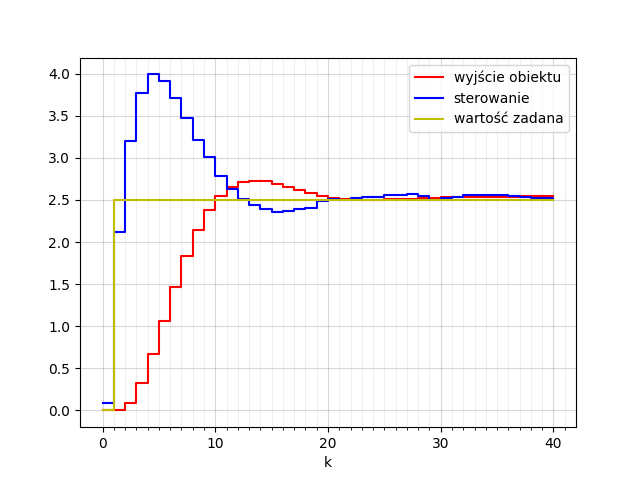
\includegraphics[width=0.7\linewidth]{regulation_net_obd_2.png}
  \caption{Regulacja do wartości zadanej 2,5 - zredukowana sieć neuronowa}
\end{figure}

\par Warto zauważyć również, że regulator oparty o sieć neuronową radzi sobie prawie bezbłędnie z utrzymaniem stałej wartości wyjścia obiektu po osiągnięciu wartości zadanej. Dla pełniejszego porównania wpływu redukcji sieci na działanie regulatora na Rysunku 5.10 przedstawiony został przebieg regulacji dla wartości zadanej 5.21. Stanowi to analogiczny przypadek do regulacji z wykorzystaniem niezredukowanej sieci neuronowej, którą widzimy na wcześniejszym rysunku 5.5. Porównując przebiegi obu symulacji należy zwrócić uwagę na dwie istotne przewagi zredukowanej sieci. Algorytm OBD pozwolił na redukcję wartości przeregulowania oraz przyczynił się do wyraźnie większej stabilności przebiegu kolejnych wartości sterujących pokazanych na wykresach niebieską linią. Wskazane korzyści jednoznacznie potwierdzają zasadność wykorzystania algorytmu OBD w trakcie nauki przez sieć neuronową zadania regulacji.
 
\begin{figure}[!h]
  \label{fig:Regulation-OBD-5}
  \centering 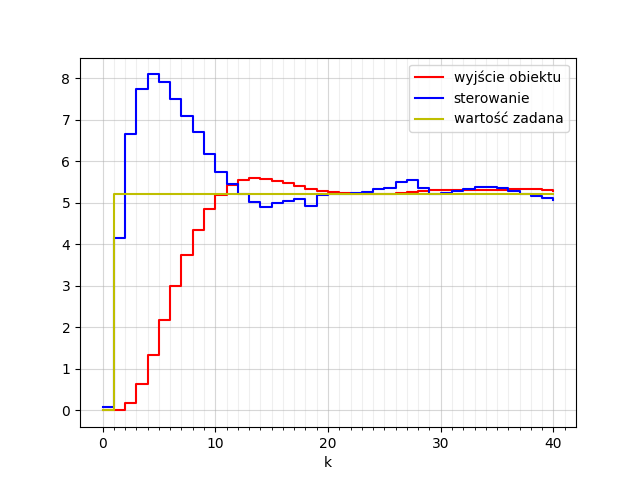
\includegraphics[width=0.7\linewidth]{regulation_net_obd_5.png}
  \caption{Regulacja do wartości zadanej 5,21 - zredukowana sieć neuronowa}
\end{figure}

\subsection{Zastosowanie innych obiektów regulacji}

\par Całość analizy przedstawionej w poprzednich podrozdziałach pozwoliła na wyselekcjonowanie i pełne wytrenowanie struktury sieci neuronowej, która w najlepszy sposób generalizuje postawione przed nią zadanie regulacji obiektu identyfikowanego przez następujące parametry \( T_1=5, \, T_2=2, \, K=1, \, T_d=0 \). Na podstawie dokonanych porównań należy stwierdzić, że regulator oparty o sieć neuronową nie posiada istotnych ograniczeń względem swojego klasycznego odpowiednika wykorzystującego metodę DMC. Jednak w realnym świecie zadanie regulacji, a co za tym idzie obiekt regulacji może charakteryzować się pewną zmiennością, która to przyczynić się może do istotnego spadku efektywności działania wykorzystywanego regulatora. Ostatnim etapem badań zaprezentowanych w tej pracy będzie zbadanie odporności danych regulatorów na modyfikacje pierwotnego obiektu regulacji. W praktyce do modyfikacji danego obiektu regulacji posłużą zmiany wcześniej ustalonych parametrów identyfikujących obiekt. Warto zauważyć, że w trakcie porównania zarówno dane, na podstawie których uczona będzie sieć jak i wektor odpowiedzi skokowej dla algorytmu DMC wyznaczany był na podstawie pierwotnego obiektu regulacji. Strategia porównania opiera się na przeprowadzeniu analogicznych symulacji jak w poprzedniej części pracy i porównaniu kolejnych błędów MSE.   

\par Pierwszy z przeprowadzonych eksperymentów dotyczył modyfikacji parametru \(T_d\). Porównano jakoś regulacji dla 5 kolejnych wartości parametru \(T_d\): 1, 2, 3, 4, 5. W przypadku każdej z tych wartości wyznaczono uśredniony bład MSE po kolejnych symulacji dla wartości zadanych z zakresu od 2 do 9. Wyniki eksperymentu zaprezentowane zostały w tabeli 5.3. Kolumna z referencyjną wartością błędu zawiera statystykę dla regulacji DMC wyznaczonej na podstawie odpowiedzi skokowej obecnego układu regulacji. Analizując kolejne wartości należy zauważyć wyraźny wzrost błędu dla obu regulatorów względem wartości referencyjnej, zwłaszcza dla wartości opóźnienia obiektu większych od dwóch. Dla pierwszego i drugiego przypadku można jednak uznać, że jakoś regulacji jest akceptowalna.  Kluczowym jest natomiast fakt, że dla każdego z przypadków błąd MSE popełniany przez regulator oparty o sieć neuronową jest zauważalnie mniejszy, a wraz z zwiększaniem opóźnienia różnica narasta. Jednoznacznie wskazuje to, że sieć neuronowa jest bardziej odporna na modyfikacje opóźnienia układu zwłaszcza w obrębie mniejszych zmian. 

\begin{table}[!h] \label{tab:tabela3} \centering
\caption{Porównanie MSE dla różnych wartości \(T_d\) zmodyfikowanego obiektu}
\begin{tabular} {| c | c | c | c |} \hline
    \(T_d\) & MSE sieć & MSE DMC & MSE referencyjne \\ \hline\hline
    1 & 3,639 & 3,668 & 3,588 \\ \hline
    2 & 4,46 & 4,827 & 4,323 \\ \hline
    3 & 5,352 & 6,593 & 5,057 \\ \hline
    4 & 6,281 & 9,277 & 5,792 \\ \hline
    5 & 7,221 & 13,490 & 6,526 \\ \hline
\end{tabular}
\end{table}

\par Dla pełniejszego obrazu postawionego twierdzenia warto przyjrzeć się przebiegom regulacji dla pierwszych dwóch przypadków. Przebiegi z wykorzystaniem dwóch metod dla kolejno parametru \(T_d\) równego 1 oraz 2 przedstawione zostały na Rysunkach 5.11-5.14. Wszystkie wykresy wyznaczone zostały dla przykładowej wartości zadanej wynoszącej 5. Na podstawie ogólnej analizy należy stwierdzić, że sieć neuronowa poradziła sobie lepiej niż regulator DMC, kluczowa jest tutaj wartość przeregulowania, która jest wyraźnie niższa zarówno dla pierwszego jak i drugiego przypadku. Jednoznacznie wskazuje to na większą odporność sieci neuronowej na zmiany opóźnienia układu względem tradycyjnego regulatora DMC. Powodów takiej zależności szukać możemy w wykorzystanej procedurze upraszczania sieci, która w założeniu sprzyjać ma generalizacji danego problemu. Ostateczna weryfikacja postawionej tezy wymagałaby jednak przeprowadzenia dalszych prac nad omawianym zagadnieniem. 

\begin{figure}[!h]
\centering
\begin{minipage}{.5\textwidth}
  \label{fig:Regulation-TD1-net}
  \centering 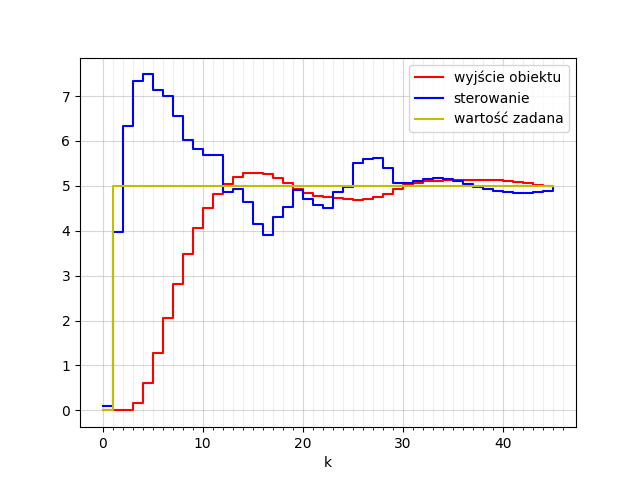
\includegraphics[width=1\linewidth]{regulation_TD1_net.png}
  \caption{Regulacja Sieć obiekt (\(T_d=1\))}
  \label{fig:test1}
\end{minipage}%
\begin{minipage}{.5\textwidth}
  \label{fig:Regulation-TD1-dmc}
  \centering 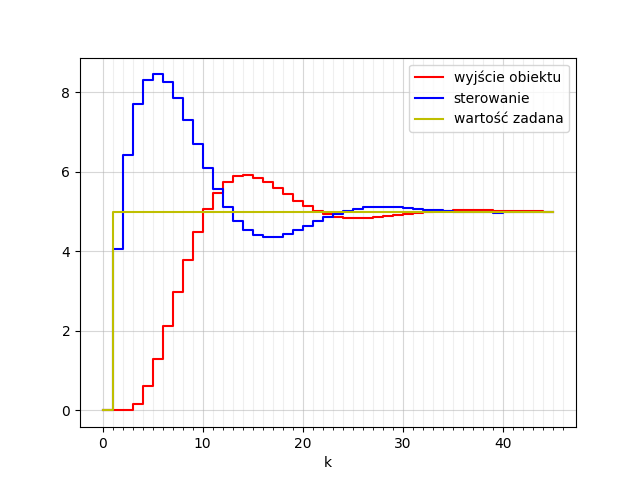
\includegraphics[width=1\linewidth]{regulation_TD1_dmc.png}
  \caption{Regulacja DMC obiekt (\(T_d=1\))}
\end{minipage}
\end{figure}

\begin{figure}[!h]
\centering
\begin{minipage}{.5\textwidth}
  \label{fig:Regulation-TD2-net}
  \centering 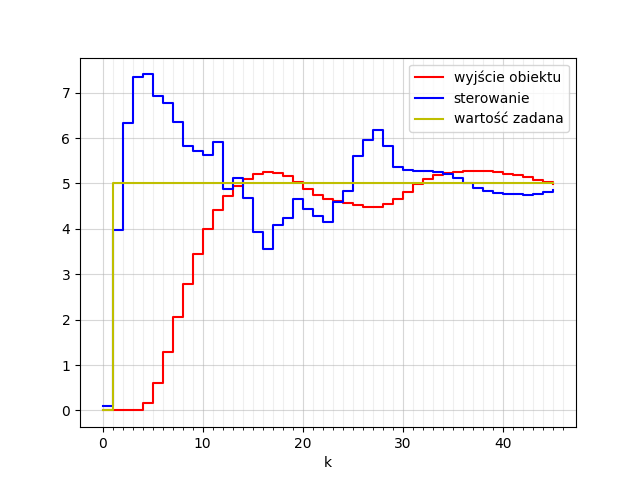
\includegraphics[width=1\linewidth]{regulation_TD2_net.png}
  \caption{Regulacja Sieć obiekt (\(T_d=2\))}
  \label{fig:test1}
\end{minipage}%
\begin{minipage}{.5\textwidth}
  \label{fig:Regulation-TD2-dmc}
  \centering 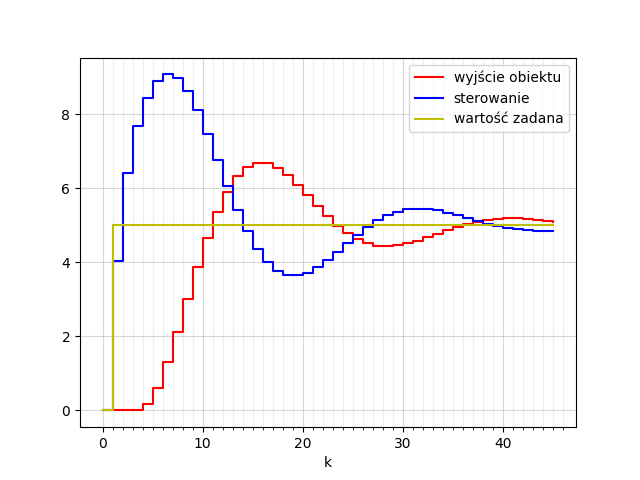
\includegraphics[width=1\linewidth]{regulation_TD2_dmc.png}
  \caption{Regulacja DMC obiekt (\(T_d=2\))}
\end{minipage}
\end{figure}

\par Kolejnym i zarazem ostatnim eksperymentem przeprowadzonym w ramach niniejszej pracy było sprawdzenie jakości regulacji dla zmodyfikowanych układów regulacji z wykorzystaniem parametrów \(T_1\) oraz \(T_2\), które początkowo wynosiły odpowiednio 5 i 2. Analizę przeprowadzono dla kilku modyfikacji, które zostały dobrane w arbitralny sposób tak aby najpełniej przedstawić możliwe warianty różnych zmian tych parametrów. Wyniki analogicznego eksperymentu do tego wykonanego wcześniej dla wpływu parametru \(T_d\) przedstawiono w Tabeli 4. Analizując przedstawione wartości błędów MSE możemy jednoznacznie stwierdzić, że obie metody regulacji są odporniejsze na zmiany parametrów \(T_1\) oraz \(T_2\) w stosunku do wcześniej prezentowanego parametru \(T_d\). Wzrost błędu MSE dla obu metod względem wartości referencyjnej jest w większości przypadków nieznaczny, a w pojedynczych przypadkach widzimy też mniejsze wartości. Jedynie w przypadku zwiększenia parametrów do wartości 7 i 6 (wiersz 5 Tabeli) rejestrujemy zauważalny wzrost wartości błędu MSE w przypadku sieci jest to wzrost o 18\% natomiast dla DMC o 20\%.     

\begin{table}[!h] \label{tab:tabela4} \centering
\caption{Porównanie MSE dla różnych wartości \(T_1\) oraz \(T_2\) zmodyfikowanego obiektu}
\begin{tabular} {| c | c | c | c | c |} \hline
    \(T_1\) & \(T_2\) & MSE sieć & MSE DMC & MSE referencyjne  \\ \hline\hline
    6 & 2 & 3,114 & 3,110 & 3,039 \\ \hline
    5 & 3 & 3,284 & 3,289 & 3,199 \\ \hline
    7 & 3 & 3,881 & 3,903 & 3,580 \\ \hline
    4 & 1 & 2,296 & 2,205 & 2,229 \\ \hline
    7 & 6 & 5,203 & 5,291 & 4,412 \\ \hline
    3 & 2 & 2,558 & 2,361 & 2,411 \\ \hline
    8 & 1 & 3,087 & 3,074 & 2,888 \\ \hline
\end{tabular}
\end{table}

\par Dla lepszego zobrazowania przedstawionych różnic warto przyjrzeć się przebiegom regulacji dla dwóch przypadków. Pierwszy z nich dotyczy parametrów \( T_1=7, \, T_2=3 \) gdy to sieć poradziła sobie lepiej ze zmianą obiektu. Rysunki 5.15 oraz 5.16 prezentują kolejno regulację z wykorzystaniem sieci neuronowej i algorytmu DMC. Główną wadą regulatora DMC w tym przypadku jest stosunkowo duża wartość przeregulowania, która nie wystąpiła przy wykorzystaniu sieci. Z drugiej strony sieć neuronowa także miała zauważalne problemy z osiągnięciem zadanej wartości.

\begin{figure}[!h]
\centering
\begin{minipage}{.5\textwidth}
  \label{fig:Regulation-T73-net}
  \centering 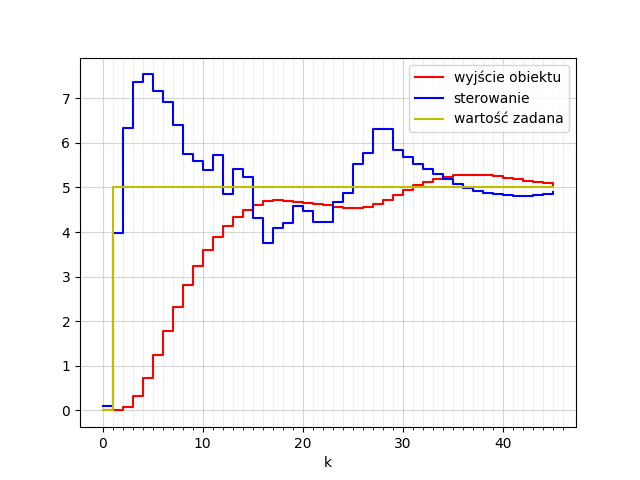
\includegraphics[width=1\linewidth]{regulation_T73_net.png}
  \caption{Regulacja Sieć obiekt (\( T_1=7, \, T_2=3 \))}
  \label{fig:test1}
\end{minipage}%
\begin{minipage}{.5\textwidth}
  \label{fig:Regulation-T73-dmc}
  \centering 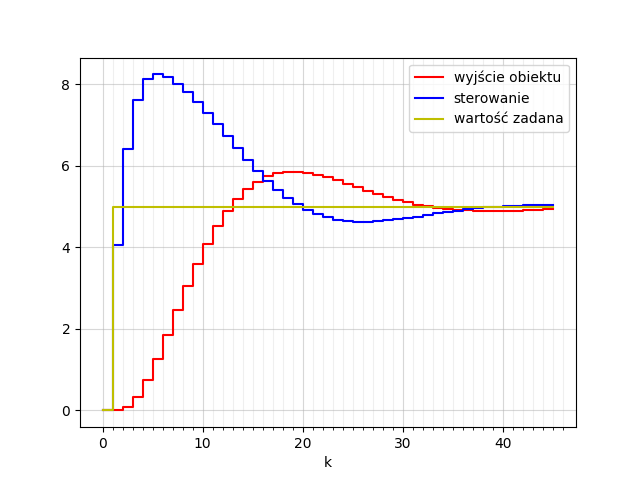
\includegraphics[width=1\linewidth]{regulation_T73_dmc.png}
  \caption{Regulacja DMC obiekt (\( T_1=7, \, T_2=3 \))}
\end{minipage}
\end{figure}

\par Drugim z prezentowanych przypadków dotyczy niższej wartość MSE dla algorytmu DMC, przykładem jest tutaj modyfikacja parametrów do wartości \( T_1=4, \, T_2=1 \). Analogiczne przebiegi regulacji względem poprzedniego punktu znajdują się na Rysunkach 5.17 i 5.18. Na wykresach odnajdujemy potwierdzenie wartości przedstawionych w tabeli, sieć neuronowa poradziła sobie gorzej z powodu występujących oscylacji wokół wartości zadanej. Regulacja oparta o algorytm DMC w tym przypadku przebiegła również z pewnymi zakłóceniami jednak należy uznać ja bliższa porządnemu efektowi. 

\begin{figure}[!h]
\centering
\begin{minipage}{.5\textwidth}
  \label{fig:Regulation-T41-net}
  \centering 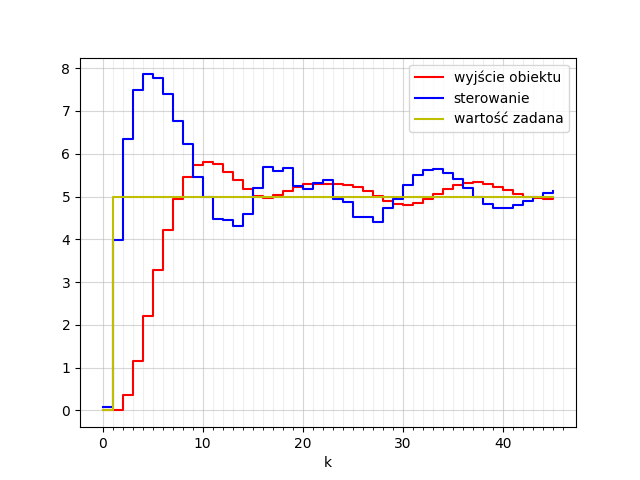
\includegraphics[width=1\linewidth]{regulation_T41_net.png}
  \caption{Regulacja Sieć obiekt (\( T_1=4, \, T_2=1 \))}
  \label{fig:test1}
\end{minipage}%
\begin{minipage}{.5\textwidth}
  \label{fig:Regulation-T41-dmc}
  \centering 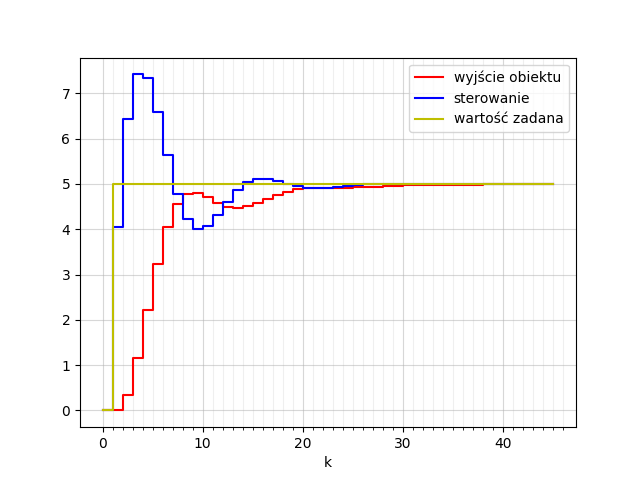
\includegraphics[width=1\linewidth]{regulation_T41_dmc.png}
  \caption{Regulacja DMC obiekt (\( T_1=4, \, T_2=1 \))}
\end{minipage}
\end{figure}

\par Przedstawione w tym podrozdziale analizy pozwalają wyciągnąć kilka istotnych wniosków. Zarówno regulatory oparte o sieci neuronowe jak i klasyczny regulator OBD są wrażliwe na zmiany obiektu regulacji. Należy jednak zauważyć, że wpływ zmian parametru opóźnienia prowadzi do wyraźnie większego zaburzenia działania obu metod w stosunku do zmian parametrów \(T_1 \) oraz \(T_2\). Pierwsza z analiz pokazała, że w obrębie małych zmian parametru \(T_d\) sieć neuronowa wykazała się większą odpornością na modyfikację układu, a uzasadnienia możemy szukać w wykorzystanej w pracy procedurze OBD. Wprawdzie jest to jedynie hipoteza, która wymaga dokładniejszej weryfikacji w czasie dalszego rozwoju zagadnienia. Nie mniej jednak wskazaną zależność należy uznać, za jedną z podstawowych przewag badanego w pracy alternatywnego podejścia względem klasycznej metody regulacji predykcyjnej. W przypadku analizy dla obiektów zmodyfikowanych poprzez parametry \(T_1 \) oraz \(T_2\) wykazane zostało, że obie metody porównywalnie dobrze radzą sobie z postawionym zagadnieniem. Nie można wskazać tutaj wyższości żadnej z metod należy jednak pamiętać, że obie z nich poradziły sobie umiarkowanie dobrze z tą klasą zmian obiektów regulacji.

\vspace{10mm}

\par Lektura niniejszego rozdziału dostarczyła czytelnikowi pełnego obrazu dokonanych eksperymentów. Szczegółowo omówiony został proces uczenia oraz upraszczania sieci. Po każdym z tych etapów porównano efektywność sieci neuronowej z klasycznym regulatorem DMC. Pod koniec przeanalizowano odporność dwóch regulatorów na zmiany obiektu regulacji. Wykazano istotne ograniczenia prezentowanych metod, a także wskazano na konkretne przypadki, w których regulacja oparta o sieć neuronową okazała się efektywniejsza. W czasie badań skupiono się na możliwie uniwersalnym podejściu dlatego wybrane zadanie regulacji może wydawać się trywialne, jednak zaprezentowane wyniki stanowić powinny wstęp do dalszej pracy nad omawianym zagadnieniem. Szczególnie interesującym może być porównanie efektywności obu metod dla wysoce dynamicznym procesów regulacji.  
